% Ensure included PDFs (banners) with newer versions embed without warnings
\pdfminorversion=7
\documentclass[aspectratio=169]{beamer}

\makeatletter
% Make LaTeX find theme .sty files in Template
\def\input@path{{../Template/}}
\makeatother
\usepackage{graphicx}
% Make graphics (including banner PDFs) resolvable without TEXINPUTS
\graphicspath{{../Template/}{../Template/banners/}{../../Common_Images/}}

%================================================================%
% Theme and Package Setup
%================================================================%
\usetheme{ucl}
\setbeamercolor{banner}{bg=darkpurple}

% Navigation and Footer
\setbeamertemplate{navigation symbols}{\vspace{-2ex}}
\setbeamertemplate{footline}[author title date]
\setbeamertemplate{slide counter}[framenumber/totalframenumber]
\setbeamertemplate{caption}{\raggedright\insertcaption\par}

\usepackage[utf8]{inputenc}
\usepackage[british]{babel} % British spelling
\usepackage{amsmath, amssymb, amsthm}
\usepackage{graphicx}
\usepackage{tikz}
\usetikzlibrary{calc, positioning, arrows.meta, shapes.geometric, trees, backgrounds, shapes.misc, graphs, quotes, shadows, fit, patterns} 
\usepackage{pgfplots}
\pgfplotsset{compat=1.17}
\usefonttheme{professionalfonts}
\usepackage{eulervm}
\usepackage{listings}
\usepackage{algorithm}
\usepackage{algpseudocode}
\usepackage{xcolor}
\usepackage{subcaption}
\captionsetup[figure]{labelformat=empty,labelsep=none}
\usepackage[export]{adjustbox}

% Define custom colours
\makeatletter
\@ifundefined{color@stone}{%
    \definecolor{stone}{gray}{0.95}%
}{}
\makeatother
\definecolor{darkgreen}{rgb}{0.0, 0.5, 0.0}
\definecolor{uclblue}{cmyk}{1,0.24,0,0.64}
\definecolor{uclred}{cmyk}{0,1,0.62,0}

\setbeamercovered{transparent}

% Define theoremblock
\makeatletter
\newenvironment<>{theoremblock}[1]{%
    \begin{block}#2{#1}%
}{\end{block}}
\makeatother

% Section divider slides
\AtBeginSection[]{
  \begin{frame}
    \frametitle{\textbf{\Large\insertsectionhead}}
    \begin{center}
        \huge\textbf{\insertsectionhead}
    \end{center}
  \end{frame}
}

% Maths Macros
\newcommand{\U}{\mathcal{U}}
\newcommand{\V}{\mathcal{V}}
\newcommand{\Z}{\mathcal{Z}}
\newcommand{\R}{\mathbb{R}}
\newcommand{\E}{\mathbb{E}}
\newcommand{\ip}[2]{\langle #1, #2 \rangle}
\newcommand{\norm}[1]{\| #1 \|}
\DeclareMathOperator*{\argmin}{argmin}
\DeclareMathOperator{\prox}{prox}
\DeclareMathOperator{\dom}{dom}
\DeclareMathOperator{\supremum}{sup}
\DeclareMathOperator{\sign}{sign}

\title{Continuous Dynamics and Variational Networks}
\subtitle{Lecture 2: Numerical Discretisation, ODENets, and Variational Networks}
\author[Martin Benning (University College London)]{Martin Benning}
\date[COMP0263]{COMP0263 -- Solving Inverse Problems with Data-Driven Models \\[1cm] 3rd March 2026}
\institute[]{University College London}

\begin{document}

% --- Title Frame ---
\begin{frame}
  \titlepage
\end{frame}

% --- Outline ---
\begin{frame}{Lecture Overview}
    \tableofcontents
\end{frame}

\section{Numerical Discretisation \& PRK Methods}

\begin{frame}{Evaluating Continuous Control computationally}
    To evaluate continuous optimal control problems computationally, we face a fundamental structural challenge regarding how we compute gradients. \vspace{1em}
    
    There are two competing paradigms in numerical optimal control:
    \begin{enumerate}
        \item \textbf{``First-discretise-then-optimise'':} Standard deep learning approach. Discretise the network into fixed layers and calculate discrete gradients via backpropagation.
        \item \textbf{``First-optimise-then-discretise'':} Derive the continuous adjoint equations first (as we did in Lecture 1 of this week), and \emph{then} discretise the resulting boundary value problem using numerical ODE solvers \cite{benning2019deep}.
    \end{enumerate}
\end{frame}

\begin{frame}{Beyond Forward Euler}
    Standard architectures like ResNets act as a \textbf{forward Euler} discretisation of an underlying ODE.
    
    \begin{itemize}
        \item \textbf{Limitation:} Forward Euler is a first-order method. It requires exceptionally small time steps (and thus, exceptionally deep networks) to achieve accurate and stable integration over a fixed horizon.
        \item \textbf{Solution:} By adopting more flexible \textbf{Runge-Kutta (RK)} methods, we achieve higher-order approximations. This allows for more complex, stable transformations with fewer active layers (stages).
    \end{itemize}
\end{frame}

\begin{frame}{Generic Runge-Kutta Methods}
    A generic $s$-stage Runge-Kutta scheme for the forward state equation $\frac{d}{dt}u = \mathcal{F}(u, \Theta)$ computes the next state $u^{l+1}$ via intermediate stages $U_i^l$:
    
    \begin{align*}
        U_i^l &= u^l + \Delta t \sum_{j=1}^s a_{i,j} \mathcal{F}(U_j^l, \Theta_j^l) \, , \quad i = 1, \dots, s \, , \\
        u^{l+1} &= u^l + \Delta t \sum_{i=1}^s b_i \mathcal{F}(U_i^l, \Theta_i^l) \, . 
    \end{align*}
    
    where $b_i$ are the weights and $a_{i,j}$ is the coefficient matrix.
\end{frame}

\begin{frame}{The Two-Point Boundary Value Problem}
    Deep learning as optimal control requires solving a coupled two-point boundary value problem:
    \begin{enumerate}
        \item Integrating the state $u(t)$ \textbf{forward} in time.
        \item Integrating the adjoint $p(t)$ \textbf{backward} in time.
    \end{enumerate}
    \vspace{1em}
    To handle this, we employ a \textbf{Partitioned Runge-Kutta (PRK)} method. This applies one RK scheme to the forward equation, and a distinct, matched RK scheme (with weights $\tilde{b}_i$ and matrix $\tilde{a}_{i,j}$) to the backward adjoint equation.
\end{frame}

\begin{frame}{Backward Runge-Kutta for the Adjoint}
    The matching backward RK scheme for the adjoint equation computes the continuous backpropagation step via intermediate stages $P_i^l$:
    
    \begin{align*}
        P_i^l &= p^l + \Delta t \sum_{j=1}^s \tilde{a}_{i,j} \ell_j^l \, , \quad i = 1, \dots, s \, , \\
        p^{l+1} &= p^l + \Delta t \sum_{i=1}^s \tilde{b}_i \ell_i^l \, , 
    \end{align*}
    
    where $\ell_i^l = -\left(\partial_u \mathcal{F}(U_i^l, \Theta_i^l)\right)^* P_i^l$ represents the stage derivatives for the adjoint state.
\end{frame}

\begin{frame}{Symplectic Partitioned Runge-Kutta}
    Remarkably, the ``first-discretise'' and ``first-optimise'' approaches \textbf{perfectly commute} if the chosen discretisation scheme is a \textbf{symplectic} PRK method \cite{hager2000runge,benning2019deep}.
    
    \begin{theoremblock}{Symplectic Conditions}
    For a PRK to be symplectic, it must preserve the discrete inner product $\langle p^{l+1}, v^{l+1} \rangle = \langle p^l, v^l \rangle$. This algebraically requires:
    $$ b_i = \tilde{b}_i \quad \text{and} \quad b_i\tilde{a}_{i,j} + \tilde{b}_j a_{i,j} - b_i\tilde{b}_j = 0 \quad \text{for all } i, j = 1, \dots, s \, . $$
    \end{theoremblock}
    
    When these hold, numerical gradients evaluated from the continuous adjoint approach match true analytical backpropagation gradients.
\end{frame}

\begin{frame}{Example: The Symplectic Euler Method}
    Consider the simplest symplectic PRK. Rather than using forward Euler for both passes, we pair the \emph{explicit} Euler for the state with the \emph{implicit} Euler for the adjoint.
    
    For a single stage ($s=1$), the forward explicitly uses $b_1 = 1, a_{1,1} = 0$.
    By the symplectic conditions, we must have
    \begin{itemize}
        \item $\tilde{b}_1 = b_1 = 1$
        \item $1 \cdot \tilde{a}_{1,1} + 1 \cdot 0 - 1 \cdot 1 = 0 \implies \tilde{a}_{1,1} = 1$ (Implicit Euler)
    \end{itemize}
    \vspace{1em}
    This pairing precisely forms the backbone of standard ResNet backpropagation, naturally preserving discrete Hamiltonian dynamics.
\end{frame}

\begin{frame}{Example: Higher-Order Explicit Methods}
    Higher-order explicit methods, such as the 2-stage Improved Euler or 4-stage Runge-Kutta, can be formulated into symplectic PRKs by algebraically deriving their corresponding backward coefficients to evaluate gradients accurately.
    
    \begin{table}[htpb]
        \centering
        \begin{tabular}{c|cc}
        0 & 0 & 0 \\ 
        1 & 1 & 0 \\ \hline
          & 1/2 & 1/2
        \end{tabular}
        \caption{Butcher tableau for the explicit 2-stage Improved Euler method.}
    \end{table}
    When used for the forward pass, a unique implicit backward tableau is derived via the symplectic conditions to ensure exact gradient matching.
\end{frame}

\section{ODENet and Learnable Time Steps}

\begin{frame}{Learnable Time Steps}
    By treating deep learning as an ODE, the ``time step'' $\Delta t$ between layers is no longer a fixed hyperparameter but can become a \textbf{learnable parameter} $\alpha$.
    
    In the \textbf{ODENet} architecture, the control set is expanded to $\Theta = (W, \beta, \alpha)$, such that the flow is given by
    $$ \mathcal{F}(u, \Theta) = \alpha \sigma(W u + \beta) \, . $$
    
    This allows the network to dynamically adjust the integration step size, effectively optimising its own depth mapping \cite{benning2019deep}.
\end{frame}

\begin{frame}{The Simplex Constraint for Sparsity}
    A powerful variation projects these learnable time steps $\alpha$ onto a probability simplex:
    $$ \mathcal{S} = \left\{ \alpha \in \mathbb{R}^N \mid \alpha^{[j]} \ge 0, \sum_j \alpha^{[j]} = 1 \right\} \, . $$
    
    \begin{itemize}
        \item This projection induces \textbf{extreme sparsity}.
        \item The network automatically sets most time steps to exactly zero.
        \item It effectively uses only few active layers to solve complex transformations, severely reducing the online memory footprint during inference.
    \end{itemize}
\end{frame}

\begin{frame}{Empirical Results: ODENets}
    Empirically, freeing time steps allows ODENets to learn complex state space transformations more aggressively, sometimes even learning non-monotonic dynamics (negative time steps).\vspace{-0.15cm}
    \begin{figure}[htpb]
        \centering
        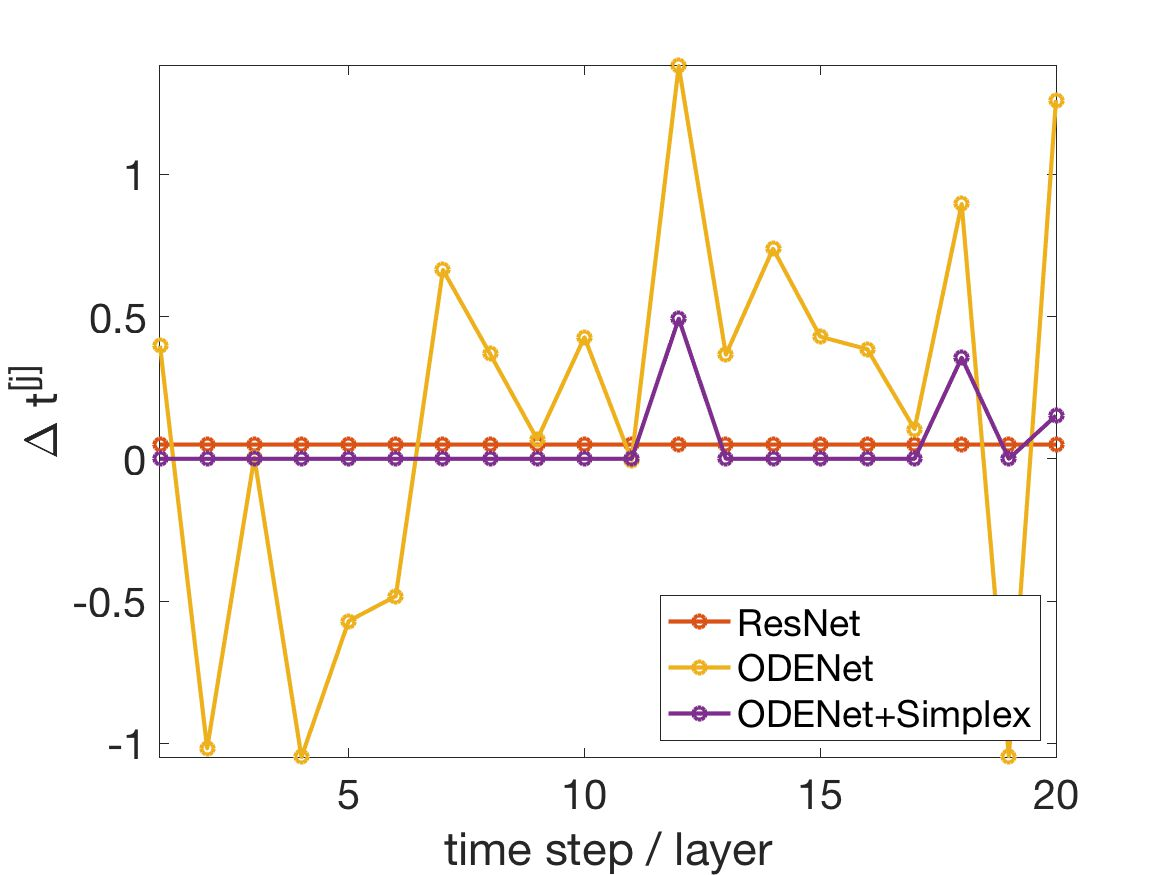
\includegraphics[width=0.4\textwidth]{../Common_Images/optimalcontrol/example_squares2d_20layers_backtracking1_seed1_timesteps}
        \caption{Learned time steps for ResNet, ODENet, and ODENet+Simplex. The simplex constraint forces the network to automatically select only a few active layers, zeroing out the rest.}
    \end{figure}
\end{frame}

\section{Variational Networks (VNs): Bridging Energy Minimisation and DL}

\begin{frame}{Reversing the ODE Perspective}
    So far, we viewed artificial networks (ResNets) as discretised ODEs to understand their stability. \vspace{1em}
    
    We can apply this perspective in \textbf{reverse}: 
    Instead of analysing a network as a dynamical system, we can \emph{derive} neural architectures directly by discretising the continuous gradient flows of established physical energy functionals. 
    \vspace{1em}
    
    This leads to \textbf{Variational Networks (VNs)} \cite{kobler2017variational,hammernik2018learning}, which are another attempt at fusing the rigorous theoretical properties of variational models with the expressiveness of deep learning.
\end{frame}

\begin{frame}{Energy Minimisation and the Field of Experts}
    Image reconstruction can be formulated as minimising an energy functional $E(u)$. By parameterising the regulariser using the \textbf{Fields of Experts (FoE)} framework, we obtain
    
    $$ E(u) = \frac{\lambda}{2} \|K u - f^\delta \|_2^2 + \sum_{i=1}^{N_D} \sum_{p=1}^N \rho_i\left((D_i u)_p\right) \, . $$
    
    \begin{itemize}
        \item $K$: Forward operator (e.g., MRI physics like the Fourier transform).
        \item $f$: Measured sensor data.
        \item $D_i$: Set of $N_D$ stacked, learned convolutional operators with corresponding filters.
        \item $\rho_i$: Learned, non-linear potential function evaluating the filter responses.
    \end{itemize}
\end{frame}

\begin{frame}{Parametrising the Potential Functions}
    To enable highly flexible, data-driven activation functions, the derivatives of the potential functions, $\rho_i^\prime$, are parametrised as a weighted sum of $M$ Gau\ss ian \textbf{Radial Basis Functions (RBFs)}, i.e.,
    
    $$ \rho_i'(x) = \sum_{j=1}^M w_{ij} \exp\left(-\frac{(x - \mu_j)^2}{2\sigma^2}\right) \, , $$
    
    where $\mu_j$ are equidistant centers and $w_{ij}$ are the learnable weights \cite{hammernik2018learning}.
\end{frame}

\begin{frame}{Incremental Gradient Steps (Unrolling)}
    To minimise the energy $E(u)$, we unroll a discrete gradient descent step. The fundamental update rule for a single Variational Network stage is:
    
    $$ u^{t+1} = u^t - \left( \sum_{i=1}^{N_D} (D_i^t)^\top \rho_i^{t\prime}(D_i^t u^t) + \lambda^t K^*(K u^t - f^\delta) \right) $$
    
    \begin{itemize}
        \item Parameters $\Theta^t = \{D_i^t, w_{ij}^t, \lambda^t\}$ can vary across each stage $t$.
        \item This structure exactly mirrors deep ResNets! The data fidelity term acts as a skip connection enforcing physics, while the regularisation term acts as a convolutional residual block.
    \end{itemize}
\end{frame}

\begin{frame}{Variational Network Architecture}
    \begin{figure}[htpb]
        \centering
        \begin{subfigure}{0.48\textwidth}
            \centering
            % Top half (trim bottom)
            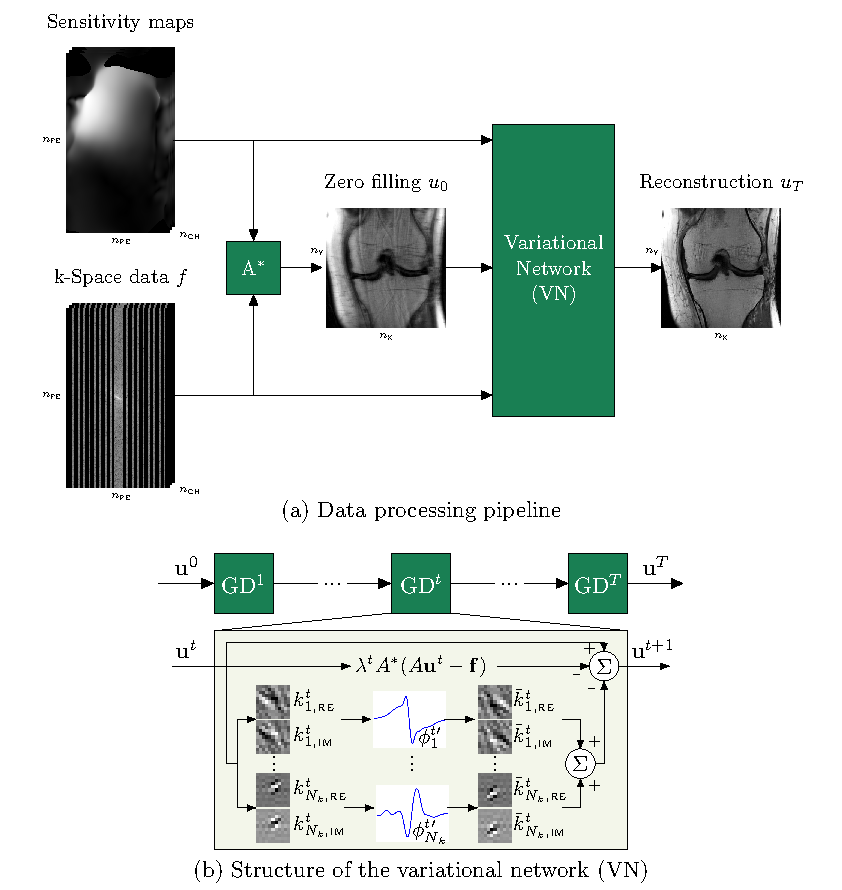
\includegraphics[trim=0 {0.82\textheight} 0 0, clip, width=\textwidth]{../Common_Images/varnetworks/figure1-vn_overview}
        \end{subfigure}\hfill
        \begin{subfigure}{0.48\textwidth}
            \centering
            % Bottom half (trim top)
            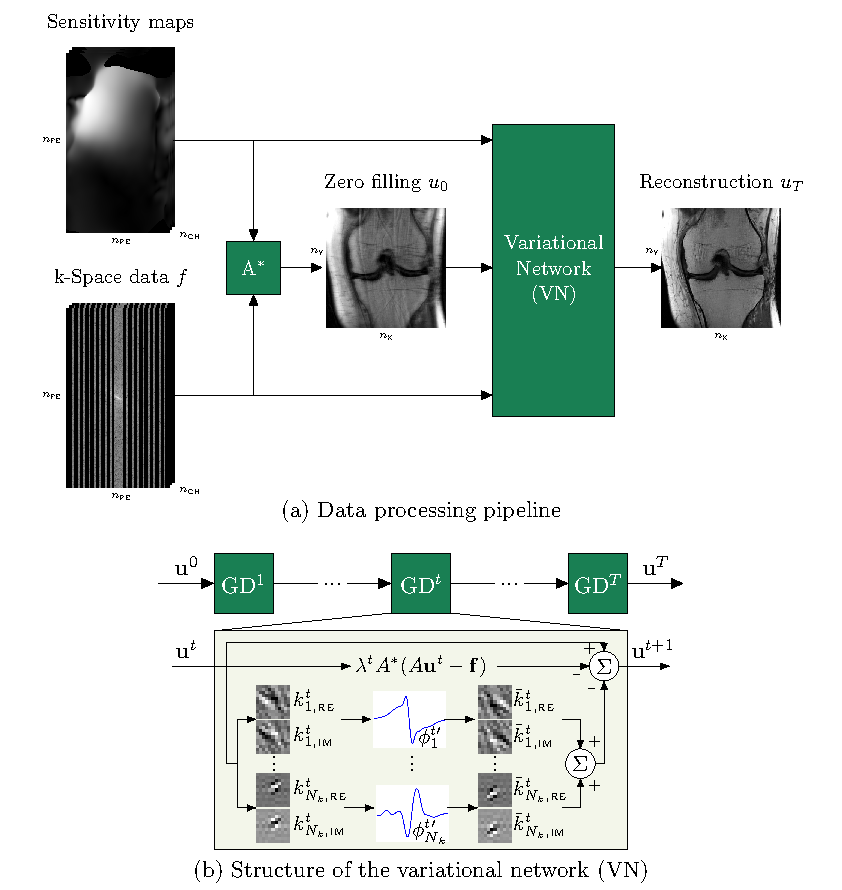
\includegraphics[trim=0 0 0 {1.3\textheight}, clip, width=\textwidth]{../Common_Images/varnetworks/figure1-vn_overview}
        \end{subfigure}
        \caption{Overview of a Variational Network. The network simulates an unrolled iterative scheme to minimise an energy functional based on the FoE regularisation functional.}
    \end{figure}
\end{frame}

\section{Clinical Applications \& The Convexity Trade-off}

\begin{frame}{Convex vs. Non-Convex Limits}
    \begin{theoremblock}{Theoretical Guarantees}
    By restricting the RBF weights to $w_{ij} > 0$ and applying zero-mean constraints to the filters $D_i$, the energy landscape $E(u)$ becomes \textbf{globally convex} \cite{kobler2017variational}.
    \end{theoremblock}
    \vspace{1em}
    \textbf{The Trade-off:}
    \begin{itemize}
        \item Convex models guarantee convergence but penalise large gradients too aggressively, leading to overly smoothed images.
        \item Highly parametrised \textbf{non-convex} VNs consistently outperform them in practice (for in-distribution samples) by capturing and preserving complex, high-frequency textures.
    \end{itemize}
\end{frame}

\begin{frame}{Application to Clinical MRI}
    When applied to multi-coil MRI data, Variational Networks must handle \textbf{complex-valued} k-space arithmetic ($u \in \mathbb{C}^N$).
    \vspace{1em}
    
    To integrate with real-valued deep learning frameworks, the network maps the complex signal into an embedded real-valued domain $\mathbb{R}^{2N}$. It splits the signal into explicit real and imaginary channels, computing independent dense filter responses before combining their magnitude \cite{hammernik2018learning}.
\end{frame}

\begin{frame}{Loss Function Design}
    To train these complex-to-real models over a dataset of $S$ pairs of undersampled clinical measurements $f_s^\delta$ and fully sampled references $u_s$, the loss function combines a robust $L_1$ norm with a complex-valued Structural Similarity Index (SSIM), i.e.,
    
    $$ \min_{\Theta} \sum_{s=1}^S \left( \| u_s - u_T(\Theta, f_s^\delta) \|_1 + \gamma \mathcal{L}_{\text{SSIM}}(u_s, u_T(\Theta, f_s^\delta)) \right) \, , $$
    
    where $\gamma > 0$ balances pixel-wise absolute differences with perceptual structure degradation.
\end{frame}

\begin{frame}{Training Overview}
    \begin{figure}[htpb]
        \centering
        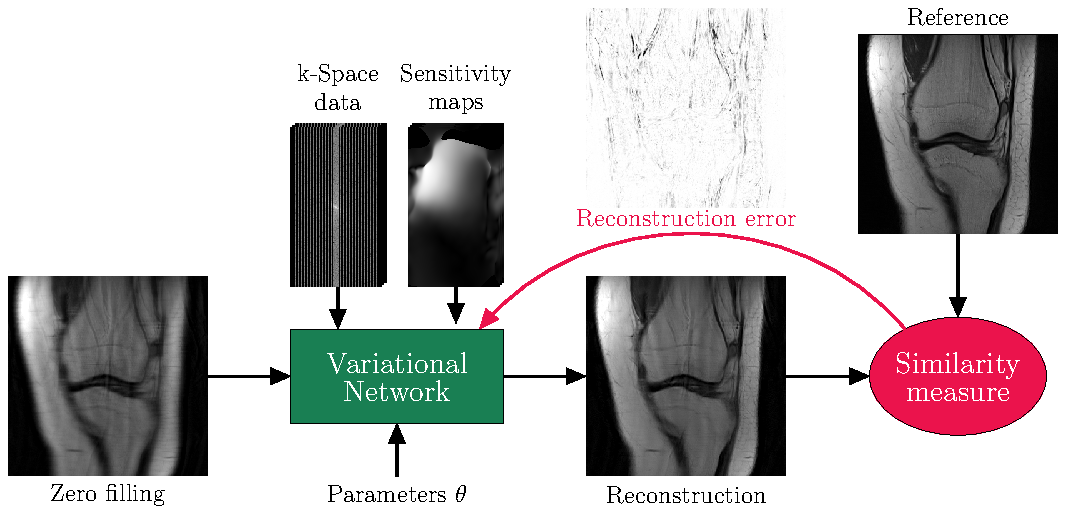
\includegraphics[width=0.75\textwidth]{../Common_Images/varnetworks/figure2-training_overview.pdf}
        \caption{Training overview for a Variational Network using paired clinical data to optimise parameters $\Theta$ over unrolled iterations \cite{hammernik2018learning}.}
    \end{figure}
\end{frame}

\begin{frame}{Interpreting Learned Filters}
    Because the unrolled layers are strictly structured as a trainable Field of Experts (FoE) regulariser, the network is highly \textbf{interpretable}.
    \vspace{1em}
    
    Reading the trained network's explicit linear filters reveals easily recognizable motifs:
    \begin{itemize}
        \item Directional Gabor-like filters.
        \item Finite-difference edge detectors.
        \item They act as non-linear, orientation-specific variants of Total Generalised Variation (TGV).
    \end{itemize}
\end{frame}

\begin{frame}{Visualising the Clinical Filters}
    \begin{figure}[htpb]
        \centering
        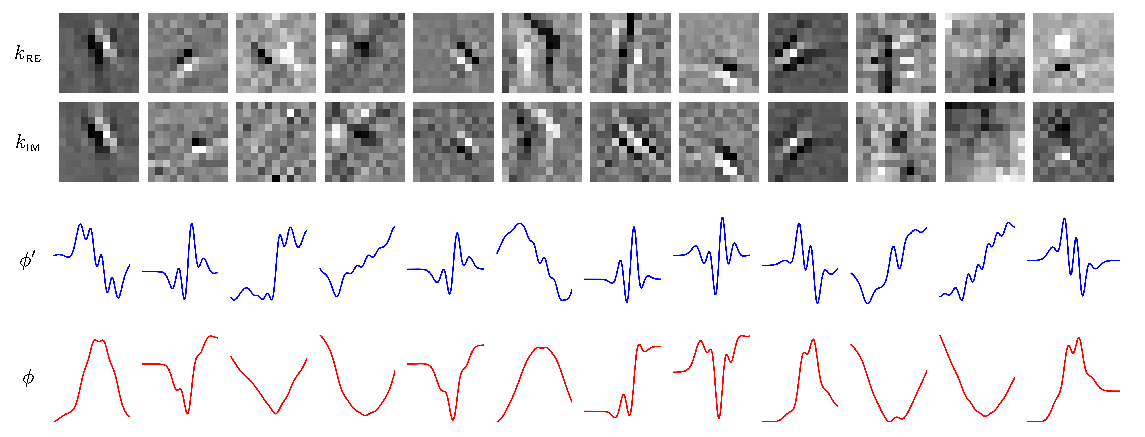
\includegraphics[width=0.8\textwidth]{../Common_Images/varnetworks/figure9-parameters.pdf}
        \caption{Visualisation of the learned complex-valued convolutional filters $D_i$ in the clinical MRI Variational Network \cite{hammernik2018learning}.}
    \end{figure}
\end{frame}

\begin{frame}{Robust Generalisation to Unseen Pathologies}
    Because the network enforces the physical forward operator $K$ at each unrolled step (via data fidelity), it avoids the aggressive hallucination phenomena commonly crippling pure black-box CNNs (like generic U-Nets).
    \vspace{1em}
    
    In clinical trials, a Variational Network restricted to just $T=10$ stages reliably reconstructed unique clinical pathologies (e.g., complex meniscal tears) that were \textbf{entirely absent} from the training dataset (cf. )\cite{hammernik2018learning}).
\end{frame}

\begin{frame}{Pathology Generalisation Example (I)}
    \begin{figure}[htpb]
        \centering
        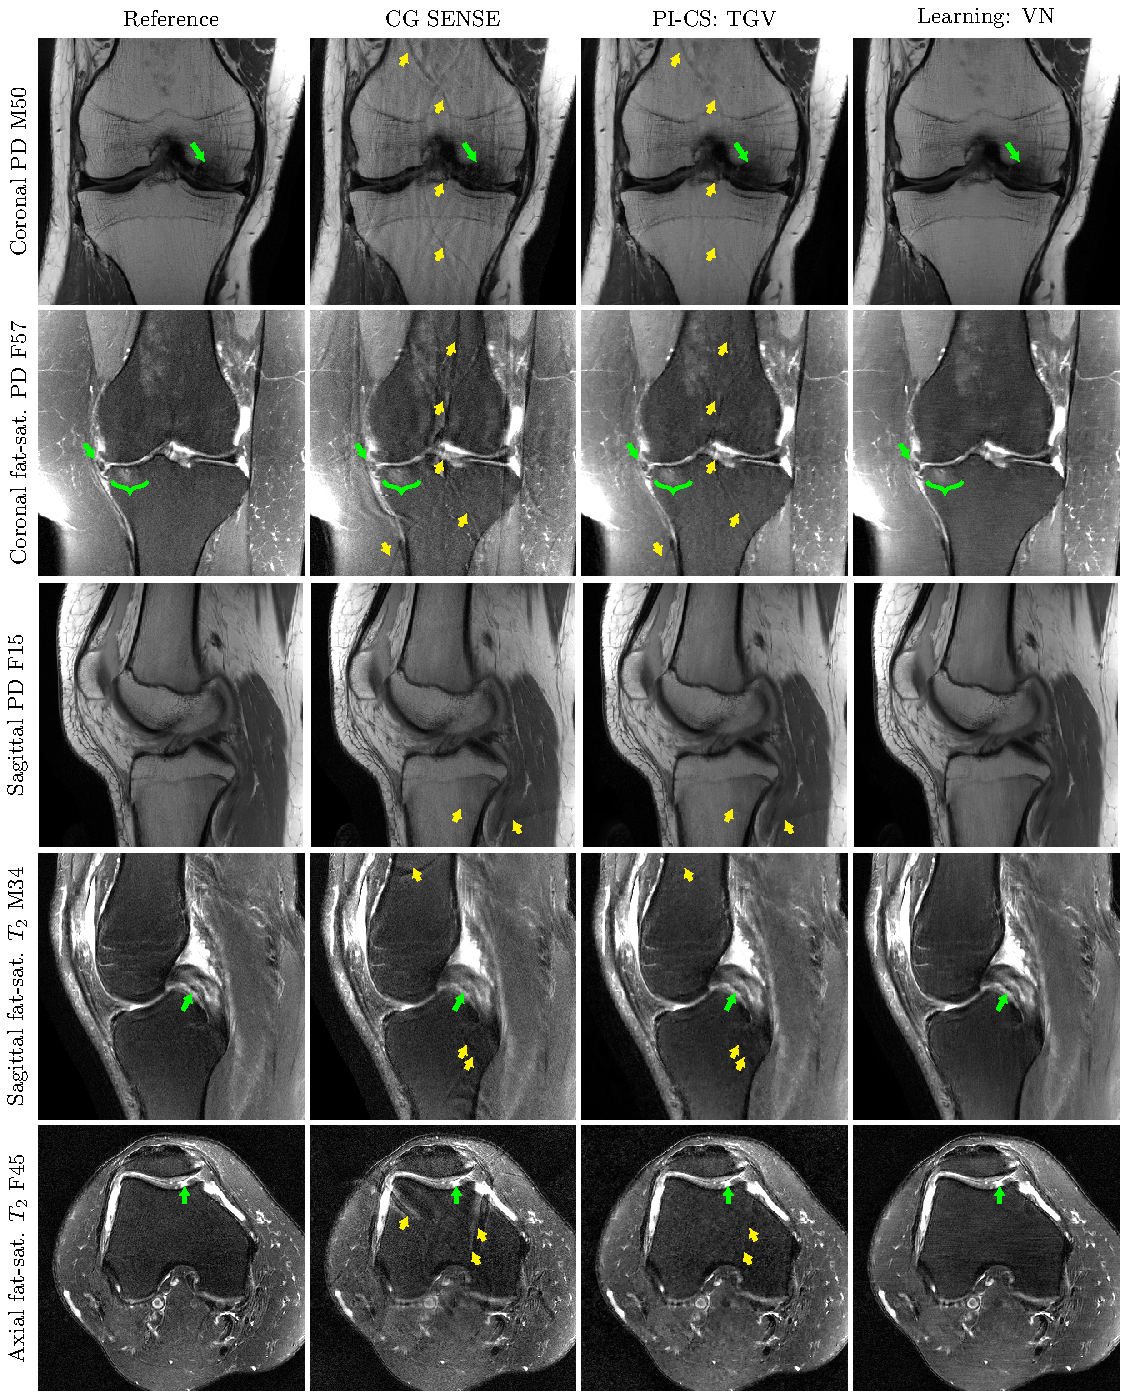
\includegraphics[trim=0 {1.97\textheight} 0 0, clip, width=0.7\textwidth]{../Common_Images/varnetworks/figure7-result_kneeprotocol.pdf}
        {\captionsetup{font=footnotesize}\caption{Despite never having seen a specific meniscal tear during training, the $T=10$ VN successfully reconstructs exact pathology, outperforming baseline U-Nets that hallucinate away unseen geometric anomalies \cite{hammernik2018learning}.}}
    \end{figure}
\end{frame}

\begin{frame}{Pathology Generalisation Example (II)}
    \begin{figure}[htpb]
        \centering
        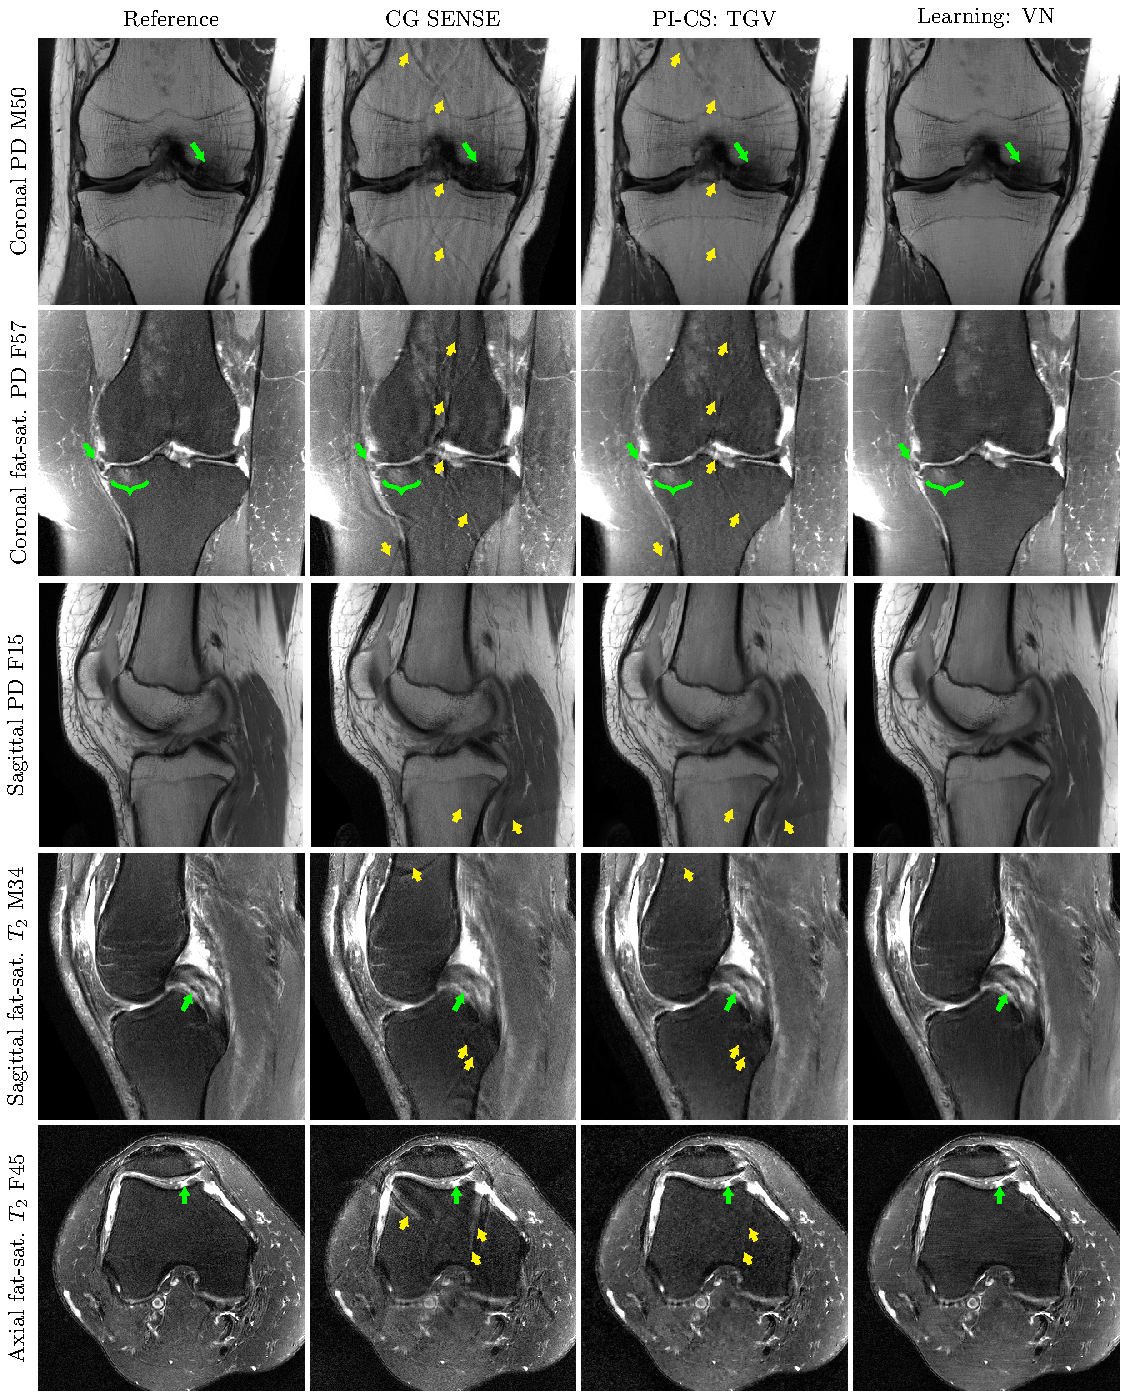
\includegraphics[trim=0 0 0 {2.05\textheight}, clip, width=0.7\textwidth]{../Common_Images/varnetworks/figure7-result_kneeprotocol.pdf}
        {\captionsetup{font=footnotesize}\caption{Despite never having seen a specific meniscal tear during training, the $T=10$ VN successfully reconstructs exact pathology, outperforming baseline U-Nets that hallucinate away unseen geometric anomalies \cite{hammernik2018learning}.}}
    \end{figure}
\end{frame}

\begin{frame}{Summary of this Lecture}
    \begin{itemize}
        \item We moved from continuous optimal control theory to \textbf{practical discretisations} using Runge-Kutta and partitioned Runge-Kutta methods.
        \item We established the \textbf{state--adjoint coupling} as a two-point boundary value problem and introduced backward RK updates for gradient evaluation.
        \item We highlighted \textbf{symplectic PRK conditions} that ensure consistency between discretise-then-optimise and optimise-then-discretise viewpoints.
        \item We introduced \textbf{ODENets} with learnable time steps and simplex constraints for sparse, efficient depth usage.
        \item We connected these ideas to \textbf{Variational Networks} for clinical MRI, including interpretability and robust pathology reconstruction.
    \end{itemize}
\end{frame}

\begin{frame}{Outlook: Next Lecture}
    In the next lecture, we examine how these variational-network dynamics behave over long optimisation horizons.
    \vspace{0.8em}
    \begin{itemize}
        \item We will analyse the \textbf{early stopping paradox}: why full convergence can degrade perceptual quality.
        \item We will connect optimisation trajectories to \textbf{modelling errors} and texture loss in inverse problems.
        \item We will derive an \textbf{optimal-control interpretation} of stopping time as a learnable design variable.
        \item We will use this perspective to motivate principled stopping strategies in variational-network reconstructions.
    \end{itemize}
\end{frame}

\begin{frame}[allowframebreaks]{References}
    \bibliographystyle{abbrv}
    \bibliography{../../Lecture_Notes/references}
\end{frame}

\end{document}